% Options for packages loaded elsewhere
\PassOptionsToPackage{unicode}{hyperref}
\PassOptionsToPackage{hyphens}{url}
%
\documentclass[
]{article}
\usepackage{lmodern}
\usepackage{amsmath}
\usepackage{ifxetex,ifluatex}
\ifnum 0\ifxetex 1\fi\ifluatex 1\fi=0 % if pdftex
  \usepackage[T1]{fontenc}
  \usepackage[utf8]{inputenc}
  \usepackage{textcomp} % provide euro and other symbols
  \usepackage{amssymb}
\else % if luatex or xetex
  \usepackage{unicode-math}
  \defaultfontfeatures{Scale=MatchLowercase}
  \defaultfontfeatures[\rmfamily]{Ligatures=TeX,Scale=1}
\fi
% Use upquote if available, for straight quotes in verbatim environments
\IfFileExists{upquote.sty}{\usepackage{upquote}}{}
\IfFileExists{microtype.sty}{% use microtype if available
  \usepackage[]{microtype}
  \UseMicrotypeSet[protrusion]{basicmath} % disable protrusion for tt fonts
}{}
\makeatletter
\@ifundefined{KOMAClassName}{% if non-KOMA class
  \IfFileExists{parskip.sty}{%
    \usepackage{parskip}
  }{% else
    \setlength{\parindent}{0pt}
    \setlength{\parskip}{6pt plus 2pt minus 1pt}}
}{% if KOMA class
  \KOMAoptions{parskip=half}}
\makeatother
\usepackage{xcolor}
\IfFileExists{xurl.sty}{\usepackage{xurl}}{} % add URL line breaks if available
\IfFileExists{bookmark.sty}{\usepackage{bookmark}}{\usepackage{hyperref}}
\hypersetup{
  pdftitle={State Space Models for Neuropsychological Cognitive Scores},
  pdfauthor={Zach Baucom, BS, zhbaucom@bu.edu; Yorghos Tripodis, PhD, yorghos@bu.edu; Michael Alosco, PhD, malsoco@bu.edu; Evan Johnson, PhD, wej@bu.edu},
  hidelinks,
  pdfcreator={LaTeX via pandoc}}
\urlstyle{same} % disable monospaced font for URLs
\usepackage[margin=1in]{geometry}
\usepackage{longtable,booktabs}
\usepackage{calc} % for calculating minipage widths
% Correct order of tables after \paragraph or \subparagraph
\usepackage{etoolbox}
\makeatletter
\patchcmd\longtable{\par}{\if@noskipsec\mbox{}\fi\par}{}{}
\makeatother
% Allow footnotes in longtable head/foot
\IfFileExists{footnotehyper.sty}{\usepackage{footnotehyper}}{\usepackage{footnote}}
\makesavenoteenv{longtable}
\usepackage{graphicx}
\makeatletter
\def\maxwidth{\ifdim\Gin@nat@width>\linewidth\linewidth\else\Gin@nat@width\fi}
\def\maxheight{\ifdim\Gin@nat@height>\textheight\textheight\else\Gin@nat@height\fi}
\makeatother
% Scale images if necessary, so that they will not overflow the page
% margins by default, and it is still possible to overwrite the defaults
% using explicit options in \includegraphics[width, height, ...]{}
\setkeys{Gin}{width=\maxwidth,height=\maxheight,keepaspectratio}
% Set default figure placement to htbp
\makeatletter
\def\fps@figure{htbp}
\makeatother
\setlength{\emergencystretch}{3em} % prevent overfull lines
\providecommand{\tightlist}{%
  \setlength{\itemsep}{0pt}\setlength{\parskip}{0pt}}
\setcounter{secnumdepth}{5}
\usepackage{booktabs}
\usepackage{longtable}
\usepackage{array}
\usepackage{multirow}
\usepackage{wrapfig}
\usepackage{float}
\usepackage{colortbl}
\usepackage{pdflscape}
\usepackage{tabu}
\usepackage{threeparttable}
\usepackage{threeparttablex}
\usepackage[normalem]{ulem}
\usepackage{makecell}
\usepackage{xcolor}
\usepackage{amsmath}
\usepackage{algorithm,algorithmic}
\addtolength{\oddsidemargin}{-.5in}%
\addtolength{\evensidemargin}{-.5in}%
\addtolength{\textwidth}{1in}%
\addtolength{\textheight}{-.3in}%
\addtolength{\topmargin}{-.8in}%
\usepackage{float}
\floatplacement{figure}{H}
\usepackage{booktabs}
\usepackage{longtable}
\usepackage{array}
\usepackage{multirow}
\usepackage{wrapfig}
\usepackage{float}
\usepackage{colortbl}
\usepackage{pdflscape}
\usepackage{tabu}
\usepackage{threeparttable}
\usepackage{threeparttablex}
\usepackage[normalem]{ulem}
\usepackage{makecell}
\usepackage{xcolor}
\ifluatex
  \usepackage{selnolig}  % disable illegal ligatures
\fi
\newlength{\cslhangindent}
\setlength{\cslhangindent}{1.5em}
\newlength{\csllabelwidth}
\setlength{\csllabelwidth}{3em}
\newenvironment{CSLReferences}[2] % #1 hanging-ident, #2 entry spacing
 {% don't indent paragraphs
  \setlength{\parindent}{0pt}
  % turn on hanging indent if param 1 is 1
  \ifodd #1 \everypar{\setlength{\hangindent}{\cslhangindent}}\ignorespaces\fi
  % set entry spacing
  \ifnum #2 > 0
  \setlength{\parskip}{#2\baselineskip}
  \fi
 }%
 {}
\usepackage{calc}
\newcommand{\CSLBlock}[1]{#1\hfill\break}
\newcommand{\CSLLeftMargin}[1]{\parbox[t]{\csllabelwidth}{#1}}
\newcommand{\CSLRightInline}[1]{\parbox[t]{\linewidth - \csllabelwidth}{#1}\break}
\newcommand{\CSLIndent}[1]{\hspace{\cslhangindent}#1}

\title{State Space Models for Neuropsychological Cognitive Scores}
\author{Zach Baucom, BS, \href{mailto:zhbaucom@bu.edu}{\nolinkurl{zhbaucom@bu.edu}} \and Yorghos Tripodis, PhD, \href{mailto:yorghos@bu.edu}{\nolinkurl{yorghos@bu.edu}} \and Michael Alosco, PhD, \href{mailto:malsoco@bu.edu}{\nolinkurl{malsoco@bu.edu}} \and Evan Johnson, PhD, \href{mailto:wej@bu.edu}{\nolinkurl{wej@bu.edu}}}
\date{}

\begin{document}
\maketitle
\begin{abstract}
Alzhemer's disease, and other related dementia diseases, are a worsening issue with an acceleration in today's aging population. Longitudinal cognitive assessment of those suffering from dementia offers vital insight into disease progression and allows for assessment of possible disease interventions. Difficulty in modeling such data arises as neuropsychological outcomes often show non-linear and heterogenous patterns of decline from patient to patient. We propose the use of state space models (SSM), specifically a Local Linear Trend (LLT) model, as an alternative to the commonly used linear mixed effect models (LMEM) for longitudinal assessments. The poroposed model includes the estimation of interpretable population linear effects on the outcome, while also allowing for subject-specific non-linearities in cognitive trajectories. To fit the LLT model we use the traditional full likelihood estimation using the Kalman Filter and Kalman Smoother. Because of computational burden and numerical inaccuracies of the full likelihood approach, we compare the use of partioned LLT and a Bayesian LLT estimation procedures. In a fully simulated data analysis, we show that the Bayesian LLT estimation procedure produces unbiased estimates, maintains proper estimate coverage, and has the highest power when compared to the LMEM and other LLT estimation procedures. We go on to show that the Bayesian LLT is unbiased and maintains proper coverage in a real data simulation analysis. Lastly, we use the LLT models to estimate the effect of the APOE e4 allele on cognitive trajectory.
\end{abstract}

{
\setcounter{tocdepth}{2}
\tableofcontents
}
\newpage{}

\hypertarget{introduction}{%
\section{Introduction}\label{introduction}}

According to the World Health Organization, dementia affects around 50 million people in the world today, with 60-70\% of those due to Alzheimer's Disease ({``Dementia''} 2020). The number of those suffering from Alzheimer's disease (AD) and Alzheimer's disease related dementia (ADRD) is only accelerating due to an increase in the aging population. Pathologically, AD is characterized by beta-amyloid neuritic plaques and accumulation of hyperphosphorylated tau (p-tau). These physical changes correspond with episodic memory and expressive language difficulties in the early stages, which then progresses to executive dysfunction, agitation, and an inability to care for one's self in the later stages ({``2021 alzheimer's disease facts and figures''} 2021). In addition to suffering experienced by those with AD, there is an added physical, emotional, and financial burden on family members and caretakers.

Much research has been done to understand how and why AD progresses in order to facilitate early detection and diagnosis, which is critical for timely implementation of intervention strategies. In particular, the National Alzheimer's Coordinating Center (NACC) is a publicly available, National Institute on Aging funded, centralized repository of harmonized data from approximately 30 Alzheimer's Disease Research Centers (ADRC) in the United States (Beekly et al. 2007). The overarching goal of the NACC is to facilitate research on AD and related diseases. Each ADRC follows a cohort of participants with and without cognitive impairment and approximately annually conducts harmonized cognitive, neuropsychiatric, and neurological evaluations. The ADRCs then deposit the harmonized data to the NACC which is compiled into large amounts of serial neuropsychological measurements. Analyzing these longitudinal outcomes provides vital insight into the disease course and presentation.

A number of challenges exist when accurately estimating effect modifiers on the neuropsychological outcomes presented in the NACC data. For interpretable results, we often rely on estimating linear effect modifiers. However, participant level cognition data are often non-linear over time and heterogeneous from subject to subject. Many participants may show a similar overall trajectory, but a given participant often shows unique patterns in their cognitive course (Rongve et al. 2016; Vik‐Mo et al. 2018). This heterogeneity can arise from unmeasured changes over time in social behavior, treatments, routines, or biologic processes that have an effect on the neuropsychological outcome.

Subject level heterogeneity in cognitive trajectories often goes unaccounted for, as is the case in studying the effect of the APOE e4 allele on cognitive decline. The APOE e4 gene has been known to be associated with Alzheimer's disease (Raber et al. 2004), but there have been conflicting publications on the effect of the allele on the rate of cognitive decline, as discussed by (Martins et al. 2005). Some studies claim no effect of the e4 allele on cognitive decline, some conclude a faster rate of decline, and a few even indicate a protective effect on the rate of decline. None of these studies seek to control for heterogeneous trajectories, which may contribute to underestimated parameter standard errors, leading to a mis-specified type I error and too many significant tests.

To better accommodate data characteristics common to neuropsychological measurements, and to estimate the effect of the APOE e4 allele on cognitive trajectory, we propose the use of a Local Linear Trend model (LLT). The LLT is a class of State Space Model (SSM) and is proposed due to its flexibility in measuring population linear effects while allowing for heterogeneous participant trajectory patterns. The SSM is traditionally a time series technique employed in situations with only a few number of participants and a large series of time points (Durbin and Koopman 2012; Fildes et al. 1991). The SSM framework has been successfully used in numerous fields such as engineering, econometrics, and health sciences. We propose its use in the situation more common to observational cognition data of a large number of participants with only a few repeated measures.

The Linear Mixed Effect Model (LMEM), which has an intuitive comparison to the LLT model, is very common when modeling neuropsychological outcomes (Feng et al. 2009; Rolland et al. 2009; Sanders et al. 2010; Stott et al. 2008). The LMEM is used due to its simple implementation and interpretation (Laird and Ware 1982), but the LMEM is typically only meant to model low order polynomials of trajectory. The LLT shares an equivalent linear effect interpretation as the LMEM, but with an added flexibility for non-linear changes in participant cognition. Some studies using the LMEM have enforced an AR(1) auto-correlation structure when modeling cognitive data to help counteract heterogeneous non-linearities (Dueck et al. 2009; Mitchell et al. 2020). Autocorrelation can be considered the effect of unobserved time-varying variables (UTV) on an outcome. Both the LMEM with an AR(1) autocorrelation and LLT make different assumptions on the behavior of the UTV. The AR(1) holds the strict assumption that the UTV effect will revert to the levels they held at an often arbitrary time of baseline. The LLT allows more flexibility in letting the UTV effect vary freely over time following a random walk process. Even with the added flexibility of the LLT, we show that it still produces accurate effect parameter estimates. Despite the advantages of the SSM, it has not been used for neuropsychological data.

Fitting a model with the traditional full likelihood LLT estimation process on a large data set can lead to extensive computation time. Estimation of the LLT model is an iterative process that includes difficult to avoid matrix inversions which increase computation exponentially as the sample size increases (Durbin and Koopman 2012). To address the computational burden of the brute force full likelihood estimation, we propose and compare a partitioned LLT and a Bayesian LLT.

The partitioned LLT randomly partitions the participants into a pre-specified number of groups then runs the traditional estimation process independently on each group. Population parameter estimates from each group are combined for more accurate population inference. By pre-specifying the maximum number of participants in a group, computation time increases linearly as the sample size increases.

The Bayesian estimation approach to the LLT model allows us to avoid large matrix inversions and instead relies on a Markov Chain Monte Carlo (MCMC) Gibb's sampling algorithm. Accurate estimation using MCMC is typically more computationally expensive for a small number of participants, but maintains a linear increase in computation, allowing it to quickly outperform the full likelihood method. Along with being the most accurate of the LLT estimation procedures, the Bayesian method can also be useful in identifying model mispecification through visual inspection of the MCMC draws.

To assess model performance we show two simulation analyses comparing the LMEM and our proposed LLTs: 1) on fully simulated data controlling the underlying data generation process and 2) on real data where the underlying data generating process is unknown.

By controlling the underlying data generation process we are able to demonstrate the LLT effectiveness under correct and incorrect model specification. The fully simulated data analysis show that the LMEMs and LLTs are unbiased, but only the LLTs maintain proper parameter coverage, even when the underlying data generating model follows that of a traditional LMEM. Maintaining proper coverage is essential for correct parameter inference.

The effectiveness of the LLT models is further showcased when we simulate using real data with an unknown underlying data generation process. Utilizing real data from the NACC we are able to show the LLT allows for proper inference of a simulated linear effect on the Animals test outcome. The LMEM with an AR(1) correlation structure fails to maintain proper parameter coverage, yielding poor results consistent with the aforementioned fully simulated analysis. The real data simulation validates that the LLTs intuitive interpretation is more realistic for neuropsycholgical outcomes.

After the proficiency of the proposed LLT is shown, we use the LMEM models and LLT models to estimate the effect of APOE e4 allele on the Animals test outcome over time. The Animals outcome, in which a participant names as many animals as possible within a minute, was chosen due its continual decline throughout dementia disease progression (Ferris and Farlow 2013).

\hypertarget{methods}{%
\section{Methods}\label{methods}}

\hypertarget{data-and-model-of-interest}{%
\subsection{Data and Model of Interest}\label{data-and-model-of-interest}}

\hypertarget{data}{%
\subsubsection{Data}\label{data}}

Data collected by the National Alzheimer's Coordinating Center (NACC) Uniform Data Set Version 2.0 (UDS, September 2014) was used to test the proposed LLT model validity. Criteria for entry into the analysis requires Alzheimer's disease participants to have transitioned from cognitively normal to mild cognitive impairment (MCI) or Dementia during the NACC follow-up period. This results in 1,269 participants with an average of 6.6 return visits (SD = 3.1) seen over a period of 6.7 years (SD = 3.4). The average transition from cognitively normal to MCI or Dementia occurs at 4.9 visits (SD = 2.8). In this sample 36.0\% of the subjects carry at least 1 APOE e4 allele. The average study participants are predominantly female (63.9\%) and of white ethnicity (87.3\%). Participants are primarily older with an average age of 77.1 years old (SD = 8.2) and have an average of 16.0 years of education (SD = 6.5).

\hypertarget{MOI}{%
\subsubsection{Model of Interest}\label{MOI}}

The Animals test outcome, in which participants have one minute to name as many animals as possible, was used as the cognitive outcome of interest (mean = 16.6, SD = 5.7). After controlling for dementia status (1 = diagnosed with MCI or dementia, 0 = otherwise), sex (1 = female, 0 = male), race (1 = white, 0 = other), age (mean centered), and education (mean centered), we wish to accurately estimate the effect of having an APOE e4 allele (1 = has at least 1 APOE e4 allele, 0 = otherwise) on the Animals test trajectory. Previous research suggests that the effect of APOE e4 status differs between males and females, therefore an interaction between e4 status and sex is included in the model. To measure the effect of the dependent variables on the Animals test trajectory, all dependent variables are put into the model as an interaction with time.

\hypertarget{proposed-model-for-neuropsychological-outcomes}{%
\subsection{Proposed Model For Neuropsychological Outcomes}\label{proposed-model-for-neuropsychological-outcomes}}

In the context of neuropsychological outcomes, the vector \(\mu_{ij}\) represents the components of subject \(i\)'s underlying cognition at observation \(j\) for \(i\in \{1, 2, ..., n\}\) and \(j \in \{1, 2, ..., J\}\). The observation \(y_{ij}\) are scores from a test aimed to measure the true underlying cognition of \(\mu_{ij}\). We propose modeling the underlying cognition \(\mu_{ij}\) broken into two components, 1.) \(\boldsymbol{\beta}\), which is a population parameter that captures the linear trajectory based on a subject's measured characteristics and 2.) \(\alpha_{ij}\), which captures subject specific random variation in cognition. This proposed model is a special case of the SMM called a Local Linear Trend Model (LLT) and can be written as,

\begin{equation}
\begin{aligned}\label{PSSM}
y_{ij} =& \alpha_{ij} + \boldsymbol{x}_{ij} \boldsymbol{\beta}_{j}
+ \varepsilon_{ij}, \ \ \  \varepsilon_{ij} \sim N(0, \sigma^2_\varepsilon)\\
\mu_{ij} =&
\begin{bmatrix}
\alpha_{ij} \\
\boldsymbol{\beta}_{j}
\end{bmatrix} = 
\begin{bmatrix}
\alpha_{i(j-1)} \\
\boldsymbol{\beta}_{j-1} 
\end{bmatrix}+ 
\begin{bmatrix}
\eta_{ij} \\
0_{p\times1}
\end{bmatrix},\ \ \ \eta_{ij} \sim N(0, \delta_{ij}\sigma^2_\eta)\\ \alpha_{i0}& \sim N(a_0, P_0),\ \  \ \boldsymbol{\beta}_0 \sim N(\boldsymbol{\beta}, 0)
\end{aligned}
\end{equation}

The row vector \(\boldsymbol{x}_{ij}\in R^{p}\) are the measured independent time varying-variables for subject \(i\) at the \(j^{th}\) observation. We assume the column vector \(\boldsymbol{\beta}_j \in R^p\) remains fixed over time and follows the same linear effect interpretation common with other linear regression methods. The linear effects of \(\boldsymbol{\beta}_j\) is a population parameter, as there is no index for subject \(i\).

The proposed model differs from traditional models in that there is a randomly varying subject specific \(\alpha_{ij}\) that follow a random walk through time. With respect to \(y_{ij}\), \(\alpha_{ij}\) follows the random walk about \(\boldsymbol{x}_{ij} \boldsymbol{\beta}_j\) and therefore can be interpreted as random variation in cognition not accounted for by the predictors \(\boldsymbol{x}_{ij}\). Notice, \(E(\alpha_{ij}|\alpha_{i(j-1)} =\tilde a_{i(j-1)}) = \tilde a_{i(j-1)}\). This indicates that the underlying variations in one's cognitive state at observation \(j\), not accounted for by the predictors \(\boldsymbol{x}_{ij}\), is centered on their underlying cognitive state at observation \(j-1\) and can freely vary up or down from that state.

The variance of the underlying state \(\alpha_{ij}\) is time dependent as the \(j^{th}\) observation can occur at any time. To accommodate unequal observation times we can adjust the variance of \(\alpha_{ij}\). Let \(t_{ij}\) be the observation time for the \(j^{th}\) observation. To adjust the variance we multiply the population variance \(\sigma^2_\eta\) with \(\delta_{ij} = t_{ij} - t_{i(j-1)}\) for observation \(j\). This adjustment allows for the estimation of the underlying variance \(\sigma^2_\eta\), even when each subject's \(\alpha_{ij}\) variance is different due to heterogeneous observation times. The freedom of variation in the subject specific cognition is much more flexible than restriction enforced in commonly used LMEM models.

A simple comparison to the LLT is a random intercept LMEM with an AR(1) auto-correlation in the errors. The LMEM AR(1) can be generalized as,

\begin{equation*}
\begin{aligned}
y_{ij} &= b_{i0}+\boldsymbol{x}_{ij}\boldsymbol{\beta}  + e_{ij}, \ \ \ b_{i0}\sim N(0, \sigma^2_b)\\
e_{ij} &=\rho e_{i(j-1)} + \epsilon_{ij}, \ \ \ \epsilon_{ij}\sim N(0, \sigma^2_\epsilon), \ \ \ \rho \in (-1,1) 
\end{aligned}
\end{equation*}

The linear effect is represented by \(\boldsymbol{\beta}\) and \(\boldsymbol{x}_{ij}\) are the covariates of subject \(i\) at observation \(j\). The value \(e_{ij}\) can be considered the underlying cognitive state at observation \(j\). If \(\rho = 1\) then \(e_{ij}\) can vary freely and this model mirrors the LLT without a measurement error on the observation equation. However, if \(|\rho| < 1\) then \(|E(e_{ij}|e_{i(j-1)} = \tilde e_{i(j-1)})|= |\rho \tilde e_{i(j-1)}| \leq |\tilde e_{i(j-1)}|\), meaning the underlying state is reverting back to the level it held at time 0. The LLT relaxes the restrictive mean reverting assumption.

\hypertarget{autocorrelation}{%
\subsubsection{Autocorrelation}\label{autocorrelation}}

Our proposed model implies a flexible dynamic moving average auto-correlation structure. Suppose \(\delta_{ij} = 1\) for all \(j\). The correlation between any two time points for subject \(i\) is defined as,

\begin{align*}
corr(y_{ij}, y_{i(j+\tau)}) = \frac{j\sigma^2_\eta + P_0}{\sqrt{\sigma^2_\varepsilon + j\sigma^2_\eta + P_0}\sqrt{\sigma^2_\varepsilon + (j+\tau)\sigma^2_\eta + P_0}}
\end{align*}

If there is no variation in \(\alpha\) over time (\(\sigma^2_\eta = 0\)) then \(corr(y_{ij}, y_{i(j+\tau)}) = \frac{P_0}{\sigma^2_\varepsilon + P_0}\). This auto-correlation structure provides an observationally equivalent parallel to a random intercept LMEM. Next, consider the reduced model of the LLT,

\begin{align*}
y_{ij} &= \alpha_{i0} + \sum^t_{j = 1} \eta_{ij} + \boldsymbol{x}_{ij} \boldsymbol{\beta}_0 + \varepsilon_{ij}
\end{align*}

If \(\sigma^2_\eta = 0\) then \(\eta_j = 0\) for \(j \in \{1, 2, ..., J\}\) then the model further reduces to,

\begin{align*}
y_{ij} &= \alpha_{i0} + \boldsymbol{x}_{ij} \boldsymbol{\beta}_0 + \varepsilon_{ij}
\end{align*}

Where \(\alpha_{i0}\sim N(a_0, P_0)\), which is directly comparable to a linear mixed effect model with a random intercept. This highlights that the proposed model can accommodate the simplistic LMEM while also accommodating more complex temporal auto-correlation.

\hypertarget{general-linear-gaussian-state-space-model}{%
\subsection{General Linear Gaussian State Space Model}\label{general-linear-gaussian-state-space-model}}

The proposed LLT model is derived from the general linear state space model. For the general linear SSM we use matrix notation and instead use the bold face vector \(\boldsymbol{y_j} = [y_{1j}, y_{2j}, ..., y_{nj}]'\) as the outcome and \(\boldsymbol{\mu_j} = [\mu_{1j}, \mu_{2j}, ..., \mu_{qj}]'\) as the latent state. A general linear state space model can be denoted as:

\begin{equation}
\begin{aligned}\label{GSSM}
\boldsymbol{y_j} &= \boldsymbol{F_j}\boldsymbol{\mu_j} + \boldsymbol{v_j}, \ \ \ \boldsymbol{v_j} \sim N(\boldsymbol{0}, \boldsymbol{V_j})\\
\boldsymbol{\mu_j} &= \boldsymbol{G_j}\boldsymbol{\mu_{j-1}} + \boldsymbol{w_j}, \ \ \ \boldsymbol{w_j} \sim N(\boldsymbol{0},\boldsymbol{W_j}) \ \ \& \ \ \boldsymbol{\mu_0} \sim N(\boldsymbol{u}, \boldsymbol{P})
\end{aligned}
\end{equation}

Both \(\boldsymbol{v_j}\) and \(\boldsymbol{w_j}\) are independent and mutually uncorrelated. The vector \(\boldsymbol{\mu_j} \in R^q\) represents the unobserved true state of the process. To estimate \(\boldsymbol{\mu_j}\) we use the observations \(\boldsymbol{y_j}\). The observations \(\boldsymbol{y_j}\) are assumed to be a linear combination of \(\boldsymbol{\mu_j}\) after being transformed by the observation matrix \(\boldsymbol{F_j}\), which is fixed by design, plus the random noise \(\boldsymbol{v_j}\). The latent states follow a Markov Chain process where \(\boldsymbol{\mu_j}\) is a linear function of \(\boldsymbol{\mu_{j-1}}\) in the form \(\boldsymbol{G_j}\boldsymbol{\mu_{j-1}}\) with the random noise \(\boldsymbol{w_j}\). The matrix \(\boldsymbol{G_j}\) is the state transition matrix and is also assumed fixed by design. This state space model can be regarded as a Hidden Markov model with continuous latent states and continuous observations.

Here, we denote \(\boldsymbol{\hat\mu_{a|b}} = E(\boldsymbol{\mu_a}|\boldsymbol{y_1, y_2, ..., y_b})\) and \(\boldsymbol{P}_{a|b} = \text{Var}(\boldsymbol{\mu_a}|\boldsymbol{y_1, y_2, ..., y_b})\) for \(a\) and \(b\) in \(\{1, 2, ..., J\}\). With known initial parameters of underlying state \(\boldsymbol{\mu_0}\) (mean \(\boldsymbol{u}\) and variance \(\boldsymbol{P}\)) and variance parameters (\(\boldsymbol{V_j}\) and \(\boldsymbol{W_j}\)) we can utilize the Kalman Filter and Kalman Smoother to calculate \(\boldsymbol{\hat{\mu}_{j|j}} = E(\boldsymbol{\mu_j}|\boldsymbol{y_1}, \boldsymbol{y_2}, ..., \boldsymbol{y_j})\) and \(\boldsymbol{P_{j|j}} = \text{Var}(\boldsymbol{\mu_j}|\boldsymbol{y_1}, \boldsymbol{y_2}, ..., \boldsymbol{y_j})\) for \(j\) in \(\{1, 2, ..., J\}\) Durbin and Koopman (2012). The expected value and variance of the unobserved states conditioned on all the data can then be calculated by iterating backwards through the Kalman Smoother. The Kalman filter and smoother is a maximum likelihood recursive algorithm that proceeds as shown in algorithm \ref{alg:kfks}.

\begin{algorithm}
\caption{Kalman Filter and Smoother}\label{alg:kfks}
\textbf{Kalman Filter}\\ 
For $j$ in $1, 2, ..., J$:
\begin{enumerate}
  \item {Predicted state:} $\boldsymbol{\hat \mu_{j|j-1}} = \boldsymbol{G_j} \boldsymbol{\hat \mu_{j-1|j-1}}$
  \item {Predicted state covariance:} $\boldsymbol{P_{j|j-1}} = \boldsymbol{G_jP_{j-1|j-1}G_j'} + W$
  \item {Innovation covariance:} $\boldsymbol{S_j = F_jP_{j|j-1}F_j' + V}$
  \item {Kalman Gain:} $\boldsymbol{K}_j = P_{j|j-1}F_j'S^{-1}_j$
  \item {Innovation:} $\boldsymbol{\tilde{f_j} = y_j - F_j \hat \mu_{j|j-1}}$
  \item {Updated state estimate:} $\boldsymbol{\hat \mu_{j|j}} = \hat \mu_{j|j-1} + K_j \tilde f_j$
  \item {Updated state covariance:} $\boldsymbol{P_{j|j}} = (I- K_jF_j)P_{j|j-1}$
  \item {Updated innovation:} $\boldsymbol{\tilde f}_{j|j} = y_j - F_j \hat \mu_{j|j}$
\end{enumerate}
Where $\boldsymbol{\hat\mu_{0|0}} = \boldsymbol{u}$ and $\boldsymbol{P_{0|0}} = \boldsymbol{P}$.
\\
\\
\textbf{Kalman Smoother} \\ 
For $j^*$ in J, J-1, ..., 1:
\begin{enumerate}
  \item Smoothed predicted state: $\boldsymbol{\hat\mu_{j^*|J}} = \boldsymbol{\hat \mu_{j^*|j^*}} + \boldsymbol{L}_j^* (\boldsymbol{\hat \mu_{(j^*+1)|J}} - \boldsymbol{\hat \mu_{(j^*+1)|j^*})}$
  \item Smoothed predicted state covariance:  $\boldsymbol{P_{j^*|J}} = \boldsymbol{P_{j^*|j^*}} - \boldsymbol{L_{j^*} G_{(j^*+1)} P_{j^*|j^*}}$
\end{enumerate}
Where $\boldsymbol{L_{j^*} = P_{{j^*}|{j^*}} G_{({j^*}+1)}' + P^{-1}_{({j^*}+1)|{j^*}}}$. 
\end{algorithm}

Proper estimates for \(\boldsymbol{\mu_j}\) depend on correctly specifying the variance parameters \(\boldsymbol{V_j}\) and \(\boldsymbol{W_j}\). When \(\boldsymbol{V_j}\) and \(\boldsymbol{W_j}\) are unknown, these parameters can be estimated by maximizing the joint log-likelihood using the limited memory Broyden-Fletcher-Goldfarb-Shanno (L-BFGS) method Zhou and Li (2007).

\begin{align*}
\ell(V_j, W_j) = -\frac{np}{2}log(2\pi)-\frac{1}{2}\sum^t_{i=1}\big(log|\tilde S_i| + \tilde f_i` S_i^{-1} f_i)
\end{align*}

To get a final estimate of the SSM model, 1.) run the Kalman Filter and Smoother, 2.) compute and maximize the log-likelihood to estimate variance parameters, 3.) iterate between 1.) and 2.) until convergence criteria is met.

Another important aspect is correctly specifying the initial parameters of \(\boldsymbol{\mu_0}\) (mean \(\boldsymbol{u}\) and variance \(\boldsymbol{P}\)), which are often unknown. However, by giving \(\boldsymbol{\mu_0}\) an ``infinite prior'' of \(\boldsymbol{P} = \infty\) and \(\boldsymbol{u} = 0\), after only a few iterations of the Kalman Filter, our estimates \(\boldsymbol{P_{i|j}}\) converge to the values they would have taken if we would have started with the true \(\boldsymbol{P}\) and \(\boldsymbol{u}\) (Durbin and Koopman 2012).

\hypertarget{formulating-proposed-model-into-state-space-form}{%
\subsubsection{Formulating Proposed Model Into State Space Form}\label{formulating-proposed-model-into-state-space-form}}

The proposed model in equation \ref{PSSM} can be rewritten to fit in the general matrix state space model framework from equation \ref{GSSM},

\begin{align*}
\boldsymbol{y_j} = &
\begin{bmatrix}
\boldsymbol{I}_n & \boldsymbol{X_j}
\end{bmatrix}
\begin{bmatrix}
\boldsymbol{\alpha_j}\\
\boldsymbol{\beta}_j
\end{bmatrix}
+ \boldsymbol{\varepsilon_j}\\
\begin{bmatrix}
\boldsymbol{\alpha_j}\\
\boldsymbol{\beta}_j
\end{bmatrix} = &
\begin{bmatrix}
\boldsymbol{I}_{(n+p)}
\end{bmatrix}
\begin{bmatrix}
\boldsymbol{\alpha}_{j-1}\\
\boldsymbol{\beta}_{j-1}
\end{bmatrix} + 
\begin{bmatrix}
\boldsymbol{\eta_j} \\
0_{p \times 1}
\end{bmatrix}\\
\text{where,}&\\ 
\boldsymbol{F_j} =& \begin{bmatrix}
\boldsymbol{I}_n & \boldsymbol{X_j}
\end{bmatrix}, \ \ \boldsymbol{\mu_j} = \begin{bmatrix}
\boldsymbol{\alpha_j}\\
\boldsymbol{\beta}_j
\end{bmatrix}, \ \ \boldsymbol{V_j} = \sigma^2_\varepsilon \boldsymbol{I}_n, \ \ \boldsymbol{G_j} = \boldsymbol{I}_{n+p}, \ \ \boldsymbol{W_j} = 
  \sigma^2_\eta\begin{bmatrix}
diag(\boldsymbol{\delta_j}) & 0\\
0 & 0
\end{bmatrix}
\end{align*}

The Kalman Filter and Kalman Smoother along with the variance optimization as described in algorithm 1 may be calculated to get an estimate of \(\boldsymbol{\mu_{j|J}} = [\boldsymbol{\alpha}_{j|J}' \ \boldsymbol{\beta}_{j|J}']'\). Recall, we assume that \(\boldsymbol{\beta}_j\) remains constant over time, so all \(\boldsymbol{\beta}_{j|J}\) for \(j\in \{1, 2, ..., J\}\) are equal. Our estimate for the linear effect of our predictors is \(\boldsymbol{\hat\beta} =\boldsymbol{\beta}_{J|J}\) which has variance \(\boldsymbol{P_{\boldsymbol{\hat\beta}} = [P_{J|J}]}_{(n+1:n+p), (n+1:n+p)}\). If modeling assumptions are met, \(\boldsymbol{\hat\beta} \sim N(B, \boldsymbol{P_{\boldsymbol{\hat\beta}}})\) which can be used for hypothesis testing (Durbin and Koopman 2012; Kalman 1960).

\hypertarget{computational-considerations}{%
\subsection{Computational Considerations}\label{computational-considerations}}

Although putting a diffuse prior on \(\boldsymbol{\mu_{0}} = [\boldsymbol{\alpha_{0}}' \ \boldsymbol{\beta}_{0}']'\) results in theoretical niceties, it comes at the cost of computational burden. Each subject shares \(\boldsymbol{\beta}\), which is now assumed random as we let \(\boldsymbol{\beta}_0 \sim N(0, \infty)\), therefore the observations in the vector \(\boldsymbol{y_j}\) are no longer treated as independent in the Kalman Filter and Kalman Smoother. This leads to the inverse of a possibly large non-sparse matrix \(\text{Var}(\boldsymbol{Y_j}|\boldsymbol{y_{1:j-1}}) = \boldsymbol{S_j} \in R^{n\times n}\) in the Kalman Filter process for \(j \in \{1, 2, ..., J\}\). The \(\boldsymbol{S_j}\) is also needed in the calculation of the log-likelihood of the variance parameters \(\sigma^2_\varepsilon\) and \(\sigma^2_\eta\), which makes it difficult to avoid the inversion at each iteration. This computational burden is then amplified as the Kalman Filter needs to be run multiple iterations for the maximum likelihood estimation calculation of \(\sigma^2_\varepsilon\) and \(\sigma^2_\eta\) to converge. In addition to considerable computation time, inverting a large matrix \(\boldsymbol{S_j}\) can also lead to numerical inaccuracies. To overcome the issues of the full likelihood estimation process, we propose either partitioning or a Bayesian Gibb's Sampling approach.

\hypertarget{partitioning}{%
\subsection{Partitioning}\label{partitioning}}

To decrease the computational burden, we propose randomly and equally partitioning the \(n\) subjects into \(k\) groups then run the Kalman Filter and Smoother on each group independently. This will result in \(\boldsymbol{\hat\beta}^{(i)}\) and \(\boldsymbol{P^{(i)}_{\boldsymbol{\hat\beta}}}\) for \(i \in \{1, 2, ..., k\}\) independent groups. We then use \(\boldsymbol{\bar\beta} = k^{-1}\sum_{i=1}^k \boldsymbol{\hat\beta}^{(i)}\) as our estimate for \(B\). If modeling assumptions are met, \(\boldsymbol{\bar\beta} \sim N(B, k^{-2}\sum_{i=1}^k\boldsymbol{P_{\boldsymbol{\hat\beta}^{(i)}}})\) which can be used for hypothesis testing.

The partitioning method enforces a linear increase in the Kalman Filter computation time as \(n\) increases for a fixed partition group size.

\hypertarget{bayesian-gibbs-sampling}{%
\subsection{Bayesian Gibb's Sampling}\label{bayesian-gibbs-sampling}}

Computational issues arise in the full likelihood estimation because \(\boldsymbol{\beta}\) is not treated as fixed in the Kalman Filter. This issue can be avoided by treating \(\boldsymbol{\beta}\) as fixed when estimating \(\alpha\), then estimating \(\boldsymbol{\beta}\) outside of the Kalman Filter using a Bayesian Gibb's Sampler. By following this methodology, the elements of \(\boldsymbol{y}_j\) will be treated as independent in the Kalman Filter and Kalman Smoother process. Using the Bayesian Gibb's Sampling framework, under regularity conditions, a sample from the joint distribution of the unknown parameters can be created. Inference can then be made using the samples of the respective parameters.

\hypertarget{the-bayesian-llt-model}{%
\subsubsection{The Bayesian LLT Model}\label{the-bayesian-llt-model}}

In this representation we no longer index the linear effect \(\boldsymbol{\beta}\) with a time component.

\begin{equation*}
\begin{aligned}
y_{ij} &= \alpha_{ij} + \boldsymbol{x}_{ij} \boldsymbol{\beta} +\varepsilon_{ij}, \ \ \ \varepsilon_{ij} \sim N(0, \sigma^2_\varepsilon)\\
\alpha_{ij} &= \alpha_{i(j-1)} + \eta_{ij}, \ \ \ \eta_{ij}\sim N(0, \delta_{ij}\sigma^2_\eta) 
\end{aligned}
\end{equation*}

We also set the following prior distributions for the unknown parameters,

\begin{equation*}
\begin{aligned}
\boldsymbol{\alpha_0} &\sim N(\boldsymbol{u}, \boldsymbol{P_0})\\
\boldsymbol{\beta} &\sim N(\boldsymbol{\theta}, \boldsymbol{I}_p\sigma^2_\beta)\\
\sigma^2_\eta &\sim IG(a_0/2, b_0/2)\\
\sigma^2_\varepsilon &\sim IG(c_0/2,d_0/2)
\end{aligned}
\end{equation*}

\hypertarget{posterior-distributions}{%
\subsubsection{Posterior Distributions}\label{posterior-distributions}}

The conditional distribution \(\boldsymbol{\alpha_{1:n}}|\boldsymbol{y_{1:n}}, \boldsymbol{X_{1:n}}, \boldsymbol{\beta}, \sigma^2_\eta, \sigma^2_\varepsilon\) can be estimated directly from the the Kalman Filter. By conditioning on \(\boldsymbol{x}_{ij}\) and \(\boldsymbol{\beta}\), each \({y_{ij}}\) is independent for \(i \in \{1, 2, ..., n\}\) and fixed \(j\). Thus, we can run the Kalman Filter with \(\tilde y_{ij} = y_{ij} - \boldsymbol{x}_{ij} \boldsymbol{\beta}\) as the outcome in the model,

\begin{equation*}
\begin{aligned}
\tilde y_{ij} &= \alpha_{ij}  +\varepsilon_{ij}\\
\alpha_{ij} &= \alpha_{i{j-1}} + \eta_{ij}
\end{aligned}
\end{equation*}

Because each element of \(\boldsymbol{\tilde y_{j}}\) are treated as independent, it is equivalent to estimating each element \(\boldsymbol{\alpha}_{j}\) independently for each subject, resulting in a computational efficient Kalman Filter where,

\begin{equation*}
\begin{aligned}
\boldsymbol{\alpha}_{j|j-1} = \boldsymbol{\alpha}_{j-1|j-1}, \ \ \ & \boldsymbol{P_{j|j-1} = P_{j-1|j-1}} + \sigma^2_\eta\\
\boldsymbol{\alpha}_{j|j} = \boldsymbol{\alpha}_{j|j-1} + \boldsymbol{K_j} (\boldsymbol{\tilde y_j- \alpha_j^{j-1}}), \ \ \ & \boldsymbol{P_{j|j}} = (1-\boldsymbol{K_j})\boldsymbol{P_{j|j-1}}\\
\boldsymbol{K_j} = \boldsymbol{\frac{\boldsymbol{P}_{j|j-1}}{\boldsymbol{P}_{j|j-1}} + \sigma^2_\varepsilon}, \ \ \ &\boldsymbol{L}_{j-1}(\boldsymbol{\alpha}_{j|J} - \boldsymbol{\alpha}_{j|j-1})
\end{aligned}
\end{equation*}

Although we are using vectors, because of the independence each operation is done element-wise. Let \(\psi = \{\sigma^2_\eta, \sigma^2_\varepsilon, \boldsymbol{\beta}\}\), the vector of the other unknown parameters. For the posterior of \(\boldsymbol{\alpha}\) we seek to find the distribution defined by,

\begin{equation*}
\begin{aligned}
P_\psi(\boldsymbol{\alpha}_{0:J}|\boldsymbol{y}_{1:J}) &= P_\psi(\boldsymbol{\alpha}_J|\boldsymbol{y}_{1:J})P_\psi(\boldsymbol{\alpha}_{j-1}|\boldsymbol{\alpha}_J, \boldsymbol{y}_{1:J}) ...  P_\psi(\boldsymbol{\alpha}_0|\boldsymbol{\alpha}_{1:J}, \boldsymbol{y}_{1:J}.)\\
&= P_\psi(\boldsymbol{\alpha}_J|\boldsymbol{y}_{1:J})P_\psi(\boldsymbol{\alpha}_{j-1}|\boldsymbol{\alpha}_n, \boldsymbol{y}_{1:(J-1)}) ...  P_\psi(\boldsymbol{\alpha}_0|\boldsymbol{\alpha}_1)
\end{aligned}
\end{equation*}

Therefore we need the following densities for \(j\) in \(1, 2, ..., J-1\):

\begin{equation*}
\begin{aligned}
P_\psi(\boldsymbol{\alpha}_j|\boldsymbol{\alpha}_{j+1}, \boldsymbol{y}_{1:j}) \propto P_\psi(\boldsymbol{\alpha}_j| \boldsymbol{y}_{1:j})P_\psi(\boldsymbol{\alpha}_{j+1}| \boldsymbol{\alpha}_j)
\end{aligned}
\end{equation*}

From the Kalman Filter we calculated \(\boldsymbol{\alpha}_j|\boldsymbol{y}_{1:j} \sim N_\psi(\boldsymbol{\alpha}_{j|j}, \boldsymbol{P}_{j|j})\) and \(\boldsymbol{\alpha}_{j+1}|\boldsymbol{\alpha}_j \sim N_\psi(\boldsymbol{\alpha}_j, \sigma^2_\eta)\). After combining the two densities \(\boldsymbol{m}_j = E_\psi(\boldsymbol{\alpha}_j| \boldsymbol{\alpha}_{j+1},\boldsymbol{y}_{1:j}) = \boldsymbol{\alpha}_{j|j} + \boldsymbol{L}_j (\boldsymbol{\alpha}_{j+1} - \boldsymbol{\alpha}_{j+1|j})\) and \(\boldsymbol{R}_j = \text{Var}_\psi(\boldsymbol{\alpha}_j| \boldsymbol{\alpha}_{j+1},\boldsymbol{y}_{1:j})= \boldsymbol{P}_{j|j} - \boldsymbol{L}_j^2 \boldsymbol{P}_{j+1|j}\) (Shumway, Rober H. and Stoffer, David S. 2017). Because of normality, the posterior distribution for \(\boldsymbol{\alpha}_j\) is \(N(\boldsymbol{m}_j, \boldsymbol{R}_j)\).

For the backward sampling procedure we start by sampling a \(\boldsymbol{\alpha}_J^*\) from a \(N_\psi(m_J, \boldsymbol{R}_J)\), then setting \(\boldsymbol{\alpha}_J^* = \boldsymbol{\alpha}_J\) for the calculation of \(\boldsymbol{m}_{T-1}\) to then sample \(\boldsymbol{\alpha}_{T-1}^*\) from a \(N_\psi(\boldsymbol{m}_{T-1}, \boldsymbol{R}_{T-1})\). This process continues until a whole chain \(\boldsymbol{\alpha}_{0:T}^*\) has been sampled.

The posterior distribution \(\boldsymbol{\beta}\) follows a pattern more similar to multivariate Bayesian regression. With all the other parameters fixed,

\begin{equation*}
\begin{aligned}
P(\boldsymbol{\beta}|Y, \boldsymbol{\alpha}, \sigma^2_\eta, \sigma^2_\varepsilon) = \frac{P(Y, \boldsymbol{\alpha}, \sigma^2_\eta, \sigma^2_\varepsilon|\boldsymbol{\beta})P(\boldsymbol{\beta})}{P(Y, \boldsymbol{\alpha}, \sigma^2_\eta, \sigma^2_\varepsilon)}
\end{aligned}
\end{equation*}

Because \(P(Y, \boldsymbol{\alpha}, \sigma^2_\eta, \sigma^2_\varepsilon)\) is constant with respect to \(\boldsymbol{\beta}\), and \(P(\boldsymbol{\beta})\) is already defined, we focus our attention on \(P(Y, \boldsymbol{\alpha}, \sigma^2_\eta, \sigma^2_\varepsilon|\boldsymbol{\beta})\).

\begin{equation*}
\begin{aligned}
P(Y, \boldsymbol{\alpha}, \sigma^2_\eta, \sigma^2_\varepsilon|\boldsymbol{\beta}) = &P(\boldsymbol{y}_1, ..., \boldsymbol{y}_J, \boldsymbol{\alpha}_1, ..., \boldsymbol{\alpha}_J, \sigma^2_\eta, \sigma^2_\varepsilon | \boldsymbol{\beta})\\
= & P(\boldsymbol{y}_J|\boldsymbol{y}_1, ..., \boldsymbol{y}_{T-1}, \boldsymbol{\alpha}_1, ..., \boldsymbol{\alpha}_J, \sigma^2_\eta, \sigma^2_\varepsilon \boldsymbol{\beta})\\
& \times P(\boldsymbol{y}_1, ..., \boldsymbol{y}_{T-1}, \boldsymbol{\alpha}_1, ..., \boldsymbol{\alpha}_J, \sigma^2_\eta, \sigma^2_\varepsilon | \boldsymbol{\beta})\\
= & P(\boldsymbol{y}_J|\boldsymbol{\alpha}_J, \sigma^2_\varepsilon \boldsymbol{\beta})P(\boldsymbol{\alpha}_{T-1}|\boldsymbol{y}_1, ..., \boldsymbol{y}_{T-1}, \boldsymbol{\alpha}_1, ..., {\boldsymbol{\alpha}_{T-1}}, \sigma^2_\eta, \sigma^2_\varepsilon, \boldsymbol{\beta})\\
& \times P(\boldsymbol{y}_1, ..., \boldsymbol{y}_{T-1}, \boldsymbol{\alpha}_1, ..., {\boldsymbol{\alpha}_{T-1}}, \sigma^2_\eta, \sigma^2_\varepsilon | \boldsymbol{\beta})\\
= & P(\boldsymbol{y}_J|\boldsymbol{\alpha}_J, \sigma^2_\varepsilon \boldsymbol{\beta})P(\boldsymbol{\alpha}_{T-1}|{\boldsymbol{\alpha}_{T-1}}, \sigma^2_\eta)\\
& \times P(\boldsymbol{y}_1, ..., \boldsymbol{y}_{T-1}, \boldsymbol{\alpha}_1, ..., {\boldsymbol{\alpha}_{T-1}}, \sigma^2_\eta, \sigma^2_\varepsilon | \boldsymbol{\beta})\\
= &P(\sigma^2_\varepsilon)P(\sigma^2_\eta)\bigg(\prod^T_{k=0} P(\boldsymbol{\alpha}_k|\boldsymbol{\alpha}_{k-1},\sigma^2_{\eta})\bigg) \prod^T_{j=1} P(\boldsymbol{y}_j|\boldsymbol{\alpha}_j, \sigma^2_\varepsilon, \boldsymbol{\beta})\\
\propto & \prod^T_{j=1} P(\boldsymbol{y}_j|\boldsymbol{\alpha}_j, \sigma^2_\varepsilon, \boldsymbol{\beta})
\end{aligned}
\end{equation*}

For simplicity we can further write,

\begin{equation*}
\begin{aligned}
-2logP(Y, \boldsymbol{\alpha}, \sigma^2_\eta, \sigma^2_\varepsilon|\boldsymbol{\beta}) \propto & \sum^T_{j=1}\frac{ (\boldsymbol{y}_j - \boldsymbol{\alpha}_j - \boldsymbol{X}_j\boldsymbol{\beta})' (\boldsymbol{y}_j - \boldsymbol{\alpha}_j - \boldsymbol{X}_j\boldsymbol{\beta})}{\sigma^2_\varepsilon}\\
\propto & \sum^T_{j=1}\frac{-2\boldsymbol{y}_j'\boldsymbol{X}_j\boldsymbol{\beta} +2\boldsymbol{\alpha}_j'\boldsymbol{X}_j\boldsymbol{\beta} + \boldsymbol{\beta}'\boldsymbol{X}_j'\boldsymbol{X}_j\boldsymbol{\beta}}{\sigma^2_\varepsilon}\\
\propto & \frac{\boldsymbol{\beta}'\big(\sum^T_{j=1}\boldsymbol{X}_j'\boldsymbol{X}_j\big)\boldsymbol{\beta} -2\big(\sum^T_{j=1}\boldsymbol{y}_j-\boldsymbol{\alpha}_j\big)'\boldsymbol{X}_j\boldsymbol{\beta} }{\sigma^2_\varepsilon}\\
\end{aligned}
\end{equation*}

We can then find the proportionality of the prior of \(\boldsymbol{\beta}\),

\begin{equation*}
\begin{aligned}
-2logP(\boldsymbol{\beta}) \propto & \frac{(\boldsymbol{\beta} - \boldsymbol{\theta})'(\boldsymbol{\beta}-\boldsymbol{\theta})}{\sigma^2_\beta}\\
\propto & \frac{\boldsymbol{\beta}'\boldsymbol{\beta} - 2\boldsymbol{\theta}\boldsymbol{\beta}}{\sigma^2_\beta}
\end{aligned}
\end{equation*}

Thus the -2log posterior of \(\boldsymbol{\beta}\) is proportional to,

\begin{equation*}
\begin{aligned}
-2logP(\boldsymbol{\beta}|Y, \boldsymbol{\alpha}, \sigma^2_\eta, \sigma^2_\varepsilon) \propto & \frac{\boldsymbol{\beta}'\big(\sum^T_{j=1}\boldsymbol{X}_j'\boldsymbol{X}_j\big)\boldsymbol{\beta} -2\big(\sum^T_{j=1}\boldsymbol{y}_j-\boldsymbol{\alpha}_j\big)'\boldsymbol{X}_j\boldsymbol{\beta} }{\sigma^2_\varepsilon} + \frac{\boldsymbol{\beta}'\boldsymbol{\beta} - 2\boldsymbol{\theta}\boldsymbol{\beta}}{\sigma^2_\beta}\\
 \propto & \frac{\boldsymbol{\beta}'\big(\sigma^2_\beta\sum^T_{j=1}\boldsymbol{X}_j'\boldsymbol{X}_j\big)\boldsymbol{\beta} -2\sigma^2_\beta\big(\sum^T_{j=1}\boldsymbol{y}_j-\boldsymbol{\alpha}_j\big)'\boldsymbol{X}_j\boldsymbol{\beta} +\boldsymbol{\beta}'\sigma^2_\varepsilon \boldsymbol{I}_p \boldsymbol{\beta} - 2\sigma^2_\varepsilon\boldsymbol{\theta}\boldsymbol{\beta}}{\sigma^2_\varepsilon\sigma^2_\beta}\\
  \propto & \frac{\boldsymbol{\beta}'\big(\sigma^2_\beta\sum^T_{j=1}\boldsymbol{X}_j'\boldsymbol{X}_j\big)\boldsymbol{\beta}+\boldsymbol{\beta}'\sigma^2_\varepsilon \boldsymbol{I}_p \boldsymbol{\beta} -2\sigma^2_\beta\big(\sum^T_{j=1}\boldsymbol{y}_j-\boldsymbol{\alpha}_j\big)'\boldsymbol{X}_j\boldsymbol{\beta}  - 2\sigma^2_\varepsilon\boldsymbol{\theta}\boldsymbol{\beta}}{\sigma^2_\varepsilon\sigma^2_\beta}\\
\propto & \frac{\boldsymbol{\beta}' \bigg(\big(\sigma^2_\beta\sum^T_{j=1}\boldsymbol{X}_j'\boldsymbol{X}_j\big)+\sigma^2_\varepsilon \boldsymbol{I}_p \bigg) \boldsymbol{\beta} -2\bigg(\sigma^2_\beta\big(\sum^T_{j=1}\boldsymbol{y}_j-\boldsymbol{\alpha}_j\big)'\boldsymbol{X}_j -\sigma^2_\varepsilon\boldsymbol{\theta}'\bigg)\boldsymbol{\beta}}{\sigma^2_\varepsilon\sigma^2_\beta}\\
\propto & \frac{(\boldsymbol{\beta} - \boldsymbol{\Sigma}^{-1} B)'
\boldsymbol{\Sigma}
(\boldsymbol{\beta} - \boldsymbol{\Sigma}^{-1}B)}{\sigma^2_\varepsilon\sigma^2_\beta}\\
\end{aligned}
\end{equation*}

Where \(B = \sigma^2_\beta\big(\sum^T_{j=1}\boldsymbol{y}_j-\boldsymbol{\alpha}_j\big)'\boldsymbol{X}_j -\sigma^2_\varepsilon\boldsymbol{\theta}'\) and \(\boldsymbol{\Sigma} = \big(\sigma^2_\beta\sum^T_{j=1}\boldsymbol{X}_j'\boldsymbol{X}_j\big)+\sigma^2_\varepsilon \boldsymbol{I}_p\). Therefore, \(\boldsymbol{\beta}|Y, \boldsymbol{\alpha}, \sigma^2_\eta, \sigma^2_\varepsilon \sim N(\boldsymbol{\Sigma}^{-1}B, \sigma^2_\varepsilon\sigma^2_\beta\boldsymbol{\Sigma}^{-1})\).

Note, \(\boldsymbol{\Sigma}\) is a \(p\times p\) matrix that needs to be inverted. If \(p\) is large, this can greatly slow down the Gibb's Sampler, especially when considering we may do several thousand iterations. However, \(\boldsymbol{\Sigma}\) can be broken down to increase computation speed. Recall, \(\boldsymbol{\Sigma} = (\big(\sigma^2_\beta\sum^T_{j=1}\boldsymbol{X}_j'\boldsymbol{X}_j\big)+\sigma^2_\varepsilon \boldsymbol{I}_p)\). The term \((\sigma^2_\beta\sum^T_{j=1}\boldsymbol{X}_j'\boldsymbol{X}_j\big)\) will not change at each iteration because it does not contain unknown parameters. By calculating the eigenvalue decomposition on \(\sigma^2_\beta\sum^T_{j=1}\boldsymbol{X}_j'\boldsymbol{X}_j\) we can rewrite \(\boldsymbol{\Sigma}\) as follows,

\begin{align*}
(\big(\sigma^2_\beta\sum^T_{j=1}\boldsymbol{X}_j'\boldsymbol{X}_j\big) + \sigma^{2}_\varepsilon \boldsymbol{I}) &=
( \boldsymbol{Q}\boldsymbol{\Lambda} \boldsymbol{Q}' + \sigma^{2}_\varepsilon \boldsymbol{I})\\
&=
( \boldsymbol{Q}\boldsymbol{\Lambda} \boldsymbol{Q}' + \sigma^{2}_\varepsilon \boldsymbol{Q}\boldsymbol{Q}')\\
&=
\boldsymbol{Q}(\boldsymbol{\Lambda} + \sigma^{2}_\varepsilon \boldsymbol{I})\boldsymbol{Q}'\\
\text{then,}\\
(\big(\sigma^2_\beta\sum^T_{j=1}\boldsymbol{X}_j'\boldsymbol{X}_j\big)+ \sigma^{2}_\varepsilon \boldsymbol{I})^{-1} &=
\boldsymbol{Q}\big(1/(\boldsymbol{\Lambda} + \sigma^{2}_\varepsilon \boldsymbol{I})\big) \boldsymbol{Q}'
\end{align*}

We only need to calculate the eigen vectors \(\boldsymbol{Q}\) and eigen values \(\boldsymbol{\Lambda}\) of \(\sigma^2_\beta\sum^T_{j=1}\boldsymbol{X}_j'\boldsymbol{X}_j\) once, then simply update \(\sigma^2_\varepsilon\) before calculating the inverse.

For the variance parameter \(\sigma^2_\eta\), we apply the same Bayes' rule rationale,

\begin{equation*}
\begin{aligned}
P(\sigma^2_\eta|Y, \boldsymbol{\beta}, \boldsymbol{\alpha}, \sigma^2_\varepsilon) =& \frac{P(Y, \boldsymbol{\beta}, \boldsymbol{\alpha}, \sigma^2_\varepsilon|\sigma^2_\eta)P(\sigma^2_\eta)}{P(Y, \boldsymbol{\beta}, \boldsymbol{\alpha}, \sigma^2_\varepsilon)}\\
\propto & P(Y, \boldsymbol{\beta}, \boldsymbol{\alpha}, \sigma^2_\varepsilon|\sigma^2_\eta)P(\sigma^2_\eta)\\
\propto & (\delta_j\sigma^2_\eta)^{-nT/2} e^{\sum^T_{j=1} (\boldsymbol{\alpha}_j-\boldsymbol{\alpha}_{j-1})^2/2\delta_j\sigma^2_\eta}(\sigma^2_\eta)^{-a_0/2-1}e^{-b_0/2\sigma^2_\eta}\\
\propto & (\sigma^2_\eta)^{-(nT+a_0)/2-1} e^{(\sum^T_{j=1} (\boldsymbol{\alpha}_j-\boldsymbol{\alpha}_{j-1})^2/\delta_j+b_0)/2\sigma^2_\eta}
\end{aligned}
\end{equation*}

Therefore, \(\sigma^2_\eta|Y, \boldsymbol{\beta}, \boldsymbol{\alpha}, \sigma^2_\varepsilon \sim IG(\frac{nT+a_0}{2}, \frac{\sum^T_{j=1} (\boldsymbol{\alpha}_j-\boldsymbol{\alpha}_{j-1})^2/\delta_j+b_0}{2})\).

In a very similar fashion we can show \(\sigma^2_\varepsilon|Y, \boldsymbol{\beta}, \boldsymbol{\alpha}, \sigma^2_\eta \sim IG(\frac{nT+c_0}{2}, \frac{d_0 + \sum^T_{j=1}(\boldsymbol{y}_j-\boldsymbol{X}_j\boldsymbol{\beta}-\boldsymbol{\alpha}_j)^2}{2})\).

\begin{algorithm}
\caption{Gibb's Sampling Algorithm}\label{alg:gibbs}
\begin{enumerate}
\item Select prior parameters $\boldsymbol{\theta}, \sigma^2_\beta, a_0, b_0, c_0, d_0$.
\item Let $\boldsymbol{\beta}^{(0)} = \boldsymbol{\theta}$, $\sigma^{2(0)}_\eta = \frac{d_0/2}{1+c_0/2}$, and $\sigma^{2(0)}_\varepsilon = \frac{b_0/2}{1+a_0/2}$.
\item Repeat steps 4-7 for $i\in\{1, 2, ..., M\}$
  \item Run a forward-filtering backward sampling procedure, conditioning on $\boldsymbol{\beta} = \boldsymbol{\beta}^{i-1}, \sigma^{2}_\eta = \sigma^{2(i-1)}_\eta, \sigma^{2}_\varepsilon =\sigma^{2(i-1)}_\varepsilon$ to get samples $\boldsymbol{\alpha}^*$, then set $\boldsymbol{\alpha}^{(i)} = \boldsymbol{\alpha}^*$.
  \item Sample $\sigma^{2*}_\eta$ from $IG(\frac{nT+a_0}{2}, \frac{\sum^T_{j=1} (\boldsymbol{\alpha}^{(i)}_j-\boldsymbol{\alpha}^{(i)}_{j-1})^2+b_0}{2})$ and set $\sigma^{2(i)}_\eta = \sigma^{2*}_\eta$.
  \item Sample $\sigma^{2*}_\varepsilon$ from $IG(\frac{nT+c_0}{2}, \frac{d_0 + \sum^T_{j=1}(\boldsymbol{y}_j-\boldsymbol{X}_j\boldsymbol{\beta}^{(i-1)}-\boldsymbol{\alpha}_j^{(i)})^2}{2})$ and set $\sigma^{2(i)}_\varepsilon = \sigma^{2*}_\varepsilon$.
  \item Sample $\boldsymbol{\beta}^*$ from $N(\boldsymbol{\Sigma}^{-1}B, \sigma^2_\varepsilon\sigma^2_\beta\boldsymbol{\Sigma}^{-1})$ where $\boldsymbol{\alpha} = \boldsymbol{\alpha}^{(i)}, \sigma^{2}_\eta = \sigma^{2(i)}_\eta, \sigma^{2}_\varepsilon=\sigma^{2(i)}_\varepsilon$ and set $\boldsymbol{\beta}^{(i)} = \boldsymbol{\beta}^*$.
\end{enumerate}
After steps 1-7 are completed posterior samples can be used as an empirical distribution to make parameter inference.
\end{algorithm}

Using the posterior distributions, the Gibb's sampling can be carried out as shown in algorithm \ref{alg:gibbs}. After removing the initial burn-in samples, to allow for posterior sample convergence, the rest of the samples can be used to make inference on any parameter of interest. We use the mean of the samples of \(\boldsymbol{\beta}\) as a point estimate for \(\boldsymbol{\beta}\) and take the 2.5 and 97.5 percentiles of the posterior draws as a pseudo 95\% confidence interval.

\hypertarget{model-validation}{%
\section{Model Validation}\label{model-validation}}

\hypertarget{simulation-controlling-underlying-data-generation-process}{%
\subsection{Simulation Controlling Underlying Data Generation Process}\label{simulation-controlling-underlying-data-generation-process}}

The fully simulated data analysis allows for insight into model behavior under different levels of model misspecification as well as confirming model accuracy. For this study we compare the proposed LLT methods to an LMEM with a random intercept and a random intercept LMEM with an AR(1) auto-correlation structure. Data for this simulation emulates the model of interest, using a simulated Animals test score as the outcome and simulated independent variables time, sex, education, race, age, transition to MCI or dementia, APOE status, and an APOE status by sex interaction. For each simulation, 100 participants are created. Each subject has 2 to 10 cognitive scores at possible observation times 0 through 9. The ``true'' linear effects are \(\boldsymbol{\beta} = [\)-0.343, -0.109, 0.006, 0.247, -0.031, -1.025, -0.132, 0.038\(]^T\). The values for \(\boldsymbol{\beta}\) in the simulations are the same as the model of interest (section \ref{MOI}) linear effect estimates from a multiple linear regression using the NACC data set. Under each simulation scenario the linear effects are estimated using an LMEM with random intercept, an LMEM with an AR(1) auto-correlation structure, the full likelihood LLT (FL LLT), partitioned LLT with 2 groups (Part 2), partitioned LLT with 4 groups (Part 4), partitioned LLT with 10 groups (Part 10), and the Bayesian LLT (BLLT).

When the underlying data generating process follows that of the LLT it has the form,

\begin{equation*}
\begin{aligned}
y_{ij} =  \alpha_{ij} + \boldsymbol{x}_{ij}\boldsymbol{\beta} + \varepsilon_{ij}, \ \ \ \varepsilon_{ij} \sim N(0,\sigma^2_\varepsilon \boldsymbol{I}_n)\\
\alpha_{ij} =  \alpha_{i(j-1)} + \eta_{ij}, \ \ \ \eta_{ij} \sim N(0,\sigma^2_\eta \boldsymbol{I}_n)\\
\end{aligned}
\end{equation*}

for \(i \in \{1, 2, ..., 100\}\). Multiple simulation scenarios are created by altering \(\sigma^2_\varepsilon\) and \(\sigma^2_\eta\) which will either increase or decrease the amount of auto-correlation in the data. For the LLT data generation, the variance parameters \((\sigma^2_\varepsilon, \sigma^2_\eta)\) take on the values (3, 0), (3, 1), (3, 2), (3, 3), (30, 10), and (60, 20).

When the underlying data generation process is an LMEM with an AR(1) variance structure it has the form,

\begin{equation*}
\begin{aligned}
y_{ij} &=  b_0 + \boldsymbol{x}_{ij} \boldsymbol{\beta} + \epsilon_{ij}, \ \ \ b_0 \sim N(0, \boldsymbol{I}_n)\\ 
\epsilon_{ij} &= \rho \ \epsilon_{i(j-1)} + e_{ij},\ \ \ e_{ij} \sim N(0, \boldsymbol{I}_n)
\end{aligned}
\end{equation*}

Under this scheme there are three scenarios of varying \(\rho = 0, 0.1, \text{and } 0.5\).

Each simulation scenario is repeated 1000 times. The main metrics of interest are 95\% confidence interval coverage, bias evaluation, and confidence interval length. In order to make proper inference, the 95\% confidence intervals should cover the parameter of interest approximately 95\% of the time. Proper coverage indicates proper probability of type I error, or probability of rejecting a null hypothesis given the null hypothesis is true. Once type I error is established, we typically wish to minimize the probability of type II error, or the probability of not rejecting a null hypothesis given the null hypothesis is false. To minimize probability of type II error we desire low parameter variance which corresponds to shorter confidence interval length. If type I error is maintained for an unbiased estimator, than a smaller confidence interval leads to higher power. Note, confidence interval length was chosen over the more common parameter variance because the Bayesian LLT uses an empirical pseudo 95\% confidence interval from the parameter posterior draws rather than the traditional Frequentist variance estimation.

The Bayesian LLT uses the following prior distributions,

\begin{equation*}
\begin{aligned}
\alpha_0 &\sim N(0, 10), \ \ \ &\boldsymbol{\beta} &\sim N(0, 10)\\
\sigma^2_\varepsilon &\sim IG(0.005, 0.005),  &\sigma^2_\eta &\sim IG((0.005, (0.005)
\end{aligned}
\end{equation*}

After 2,000 posterior draws for the unknown parameters, samples 1 through 1,000 are discarded as a ``burn-in'' sample and samples 1,001 through 2000 are used to make parameter inference.

\hypertarget{fully-simulated-data-results}{%
\subsubsection{Fully Simulated Data Results}\label{fully-simulated-data-results}}

The LME and LMEM with an AR(1) temporal correlation structure both maintain 95\% parameter coverage when the model is correctly specified. However, as the variance of the latent state (\(\sigma^2_\eta\)) increases there is evident under coverage. The LLTs maintain near 95\% coverage even when the underlying data generating process is that of an AR(1) with \(\rho = 0.5\), suggesting the LLT models are more robust to model misspecification.

All methods show unbiasedness under each simulation scenario. Of the state space models the Bayesian estimation process has the smallest variability in effect estimates and closely rivals that of the LMEMs. The partitioned state space model with 10 groups shows high estimate volatility, however, when there are 2 or 4 groups the estimate resemble the full data model. This suggest that if the number of estimated parameters is reasonable compared to the group size, then partitioning will decrease computation time without sacrificing much in terms of estimation.

Among the LLT methods, the Bayesian LLT estimation also maintains the smallest confidence interval length for the linear effect parameters, which translates to higher power. The LMEM methods have an even smaller confidence interval length, but because the LMEM methods do not have the correct 0.05 probability of type I error the comparison is inconsequential.

\begin{longtable}[t]{l|l|l|r|r|r|r|r|r|r}
\caption{\label{tab:unnamed-chunk-12}Combined linear effect coverage proportion. The LMEM methods fail to maintain 95 percent coverage when the true data generation process is that of an LLT. The LLT estimation procedures, however, maintain near 95 percent coverage even under model mispecification.}\\
\hline
\multicolumn{1}{c|}{\makecell[c]{Simulation\\Model}} & \multicolumn{2}{c|}{\makecell[c]{Variance\\Parameters}} & \multicolumn{2}{c|}{\makecell[c]{Traditional\\Methods}} & \multicolumn{5}{c}{State Space Methods} \\
\cline{1-1} \cline{2-3} \cline{4-5} \cline{6-10}
 &  &   & LME & AR(1) & FL LLT & Part 2 & Part 4 & Part 10 & BLLT\\
\hline
AR(1) & $\sigma^2 = 1$ & $\rho = 0$ & 0.954 & 0.953 & 0.947 & 0.952 & 0.963 & 0.983 & 0.964\\
\hline
AR(1) & $\sigma^2 = 1$ & $\rho = 0.1$ & 0.938 & 0.947 & 0.945 & 0.953 & 0.963 & 0.981 & 0.955\\
\hline
AR(1) & $\sigma^2 = 1$ & $\rho = 0.5$ & 0.889 & 0.944 & 0.965 & 0.967 & 0.977 & 0.987 & 0.962\\
\hline
LLT & $\sigma^2_\varepsilon = 3$ & $\sigma^2_\eta =0$ & 0.941 & 0.940 & 0.944 & 0.965 & 0.969 & 0.978 & 0.958\\
\hline
LLT & $\sigma^2_\varepsilon = 3$ & $\sigma^2_\eta =1$ & 0.790 & 0.847 & 0.947 & 0.948 & 0.956 & 0.972 & 0.940\\
\hline
LLT & $\sigma^2_\varepsilon = 3$ & $\sigma^2_\eta =2$ & 0.736 & 0.836 & 0.948 & 0.944 & 0.950 & 0.970 & 0.932\\
\hline
LLT & $\sigma^2_\varepsilon = 3$ & $\sigma^2_\eta =3$ & 0.715 & 0.838 & 0.946 & 0.940 & 0.945 & 0.969 & 0.928\\
\hline
LLT & $\sigma^2_\varepsilon = 30$ & $\sigma^2_\eta =10$ & 0.781 & 0.840 & 0.947 & 0.941 & 0.945 & 0.970 & 0.946\\
\hline
LLT & $\sigma^2_\varepsilon = 60$ & $\sigma^2_\eta =20$ & 0.780 & 0.840 & 0.946 & 0.944 & 0.945 & 0.967 & 0.943\\
\hline
\end{longtable}

\begin{figure}
\centering
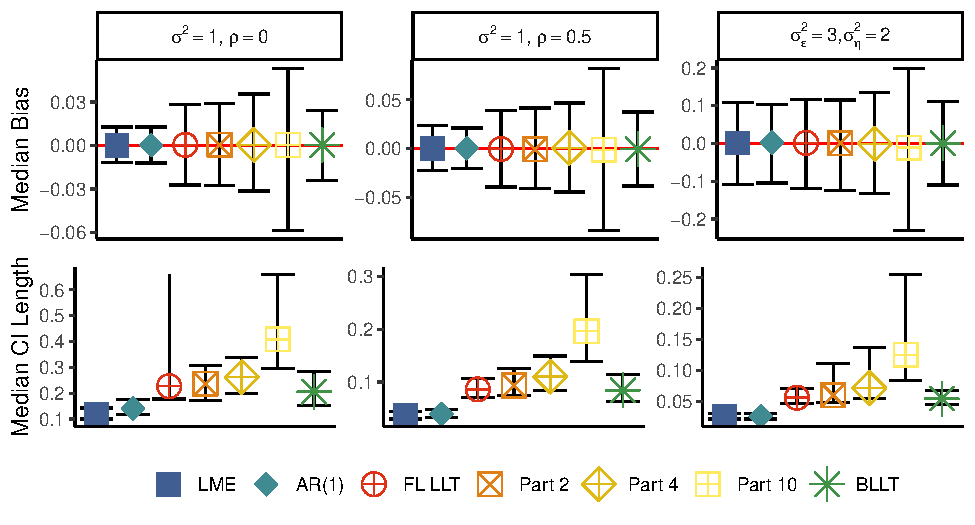
\includegraphics{Master_files/figure-latex/unnamed-chunk-15-1.pdf}
\caption{\label{fig:unnamed-chunk-15}Bias and confidence interval length with imperical 95 percent confidence interval. All estimation methods show unbiasedness. Of the LLT procedures, the Bayesian LLT has the least amount of variablity in the estimates. The LMEM methods have the smallest confidence interval length, but do not maintain 95 percent coverage. Among the methods that do cover at 95 percent (the LLTs), the Bayesian LLT has the smallest confidence interval length across the different scenarios.}
\end{figure}

\hypertarget{real-data-simulation}{%
\subsection{Real Data Simulation}\label{real-data-simulation}}

Although assessing model accuracy under correct and incorrect model specification is important, of more importance is evaluation of the models when the underlying data generation of the neuropsychological outcome is unknown. To compare the proposed LLT models and commonly used LMEMs we conduct a simulation study using the real NACC data. For each of the 1,000 simulations, half of the NACC participants are randomly selected and given a linear group effect to the existing Animals test outcome. The LLT and LME models are then used to estimate the original model of interest (section \ref{MOI}) with the additional simulated group effect. If the unknown temporal covariance structure is correctly specified by the model, we expect to accurately estimate this simulated group effect by showing unbiasedness and proper 95\% coverage. The models used to estimate the simulated group effect are a linear mixed effect model with a random intercept, a linear mixed effect model with a random intercept and AR(1) auto-correlation, partitioned LLT model with k = 50 groups, and a Bayesian LLT model.

For the NACC simulation, the Bayesian LLT model unknown parameters have the same prior distribution as is done in the full data simulation. We use the same 1,000 sample ``burn-in'' and 1,000 samples for inference as well.

\hypertarget{real-data-simulation-results}{%
\subsection{Real Data Simulation Results}\label{real-data-simulation-results}}

When estimating the randomly prescribed group effect on the Animals outcome, the partitioned LLT and Bayesian LLT methods maintain unbiasedness and proper 95\% confidence interval coverage (93.5\% and 94.0\% respectively). Both linear mixed effect models, while unbiased, did not maintain proper type I error of 0.05. The random intercept LMEM has poor coverage at 79.5\% and the random intercept LMEM with an AR(1) temporal variance structure has coverage of 88.9\%. The LMEM with the AR(1) variance structure did better than the standard LMEM on coverage, but the probability of type I error is estimated as 0.11 which is more than double the prescribed 0.05.

The coverage results from the real data simulation are consistent with results found in the full data simulation. The variance parameter estimates on the NACC data set for the Bayesian LLT are \(\hat \sigma^2_\varepsilon = 7.86\) and \(\hat \sigma^2_\eta = 2.19\) which is a 3.59 to 1 ratio. The fully simulated data coverage for the standard LMEM, the LMEM with an AR(1), and the Bayesian LLT under the scenario \(\sigma^2_\varepsilon = 3, \sigma^2_\eta = 1\) are 79.0\%, 84.7\%, and 94.0\% respectively.

\begin{longtable}[t]{l|l|l|l}
\caption{\label{tab:unnamed-chunk-18}Simulated effect parameter coverage proportion. The LMEM methods do not maintain 95 percent coverage, while the LLT estimation procedures do.}\\
\hline
LMEM & LMEM AR(1) & Partition LLT & Bayesian LLT\\
\hline
0.795 & 0.889 & 0.935 & 0.940\\
\hline
\end{longtable}

\begin{figure}
\centering
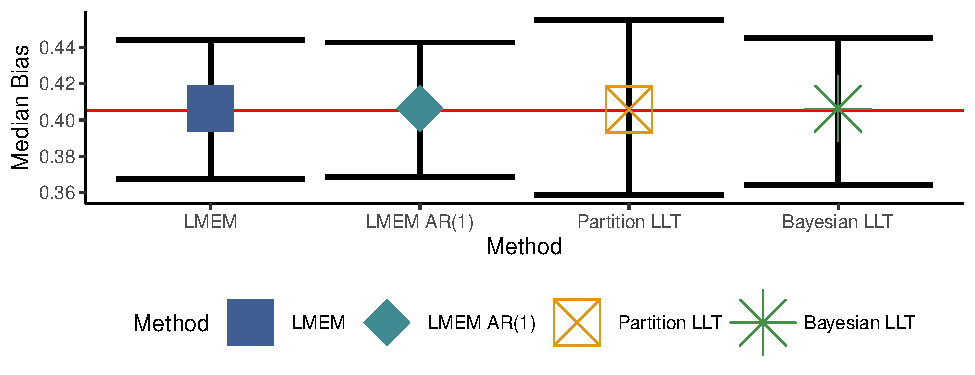
\includegraphics{Master_files/figure-latex/unnamed-chunk-19-1.pdf}
\caption{\label{fig:unnamed-chunk-19}Simulated effect parameter bias with empirical 95 percent confidence interval. All estimation methods are unbiased. The Bayesian LLT has less variability in the estimates when compard to the Partition LLT.}
\end{figure}

\hypertarget{computation-time-comparison}{%
\subsection{Computation Time Comparison}\label{computation-time-comparison}}

To compare the computation time of the full likelihood, partitioned LLT, and Bayesian LLT we simulate data with two continuous predictors, 5 repeated measurements, and a sample size of 50, 100, 200, 250, 300, 500, 750, and 1000 subjects. Estimation is carried out 1000 times for each scenario and the computation time is tracked for the 3 different model estimation processes. For the partitioned LLT we set the group size equal to 50 i.e.~for the sample size of 250, we will have 5 groups, each with size of 50. The partition of group size 50 was chosen as it showed the fastest computation time among other group sizes. The Bayesian LLT estimation used 2,000 Gibb's sampling iterations.

\hypertarget{computation-time-results}{%
\subsubsection{Computation Time Results}\label{computation-time-results}}

The full likelihood LLT estimation procedure yields an exponential increase in computation time as the sample size increases. This is due to repeatedly inverting large matrices in the Kalman Filter and Kalman Smoother algorithm. Sample sizes greater than 250 resulted in estimation failures for the full likelihood, and for this reason we only show up to n = 250 in figure \ref{fig:compTime}.

Both the partitioned LLT and the Bayesian LLT estimation procedures show a linear increase in computation time as the sample size increases. At the sample size of 50, the Bayesian LLT estimation has the longest median computation time (2.98 seconds) when compared to the full likelihood LLT (1.97 seconds) and the partitioned LLT (1.94 seconds). However, when compared to the other methods, the Bayesian LLT also has the lowest rate of change in computation time as the sample size increases. At the sample size of 150, the Bayesian method maintains faster computation time (5.02 seconds) than the full likelihood (13.77 seconds) and partitioned (5.57 seconds) LLTs. For each subsequent sample size, the Bayesian method outperforms the other methods.

\begin{figure}
\centering
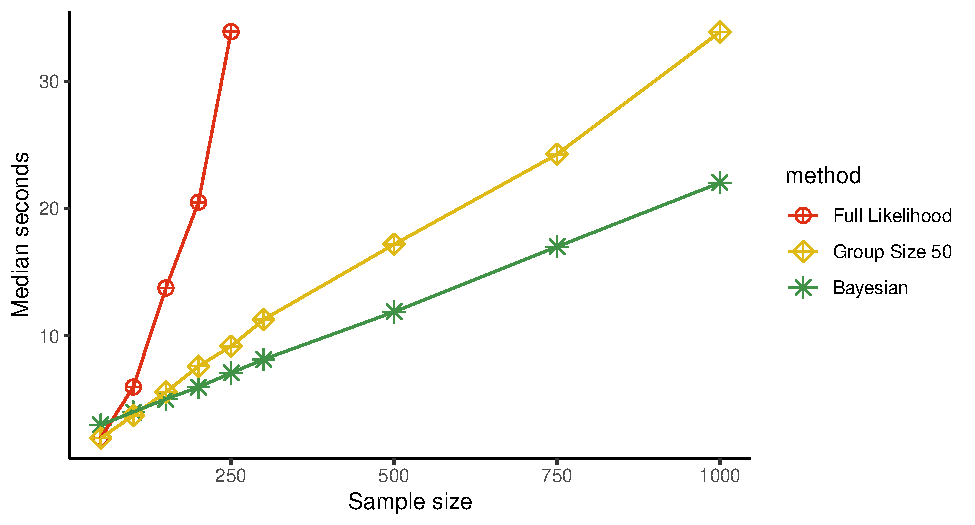
\includegraphics{Master_files/figure-latex/compTime-1.pdf}
\caption{\label{fig:compTime}Computation time comparison. As the sample size increases, the Bayesian estimation has the shortest computation time compared to the other estimation procedures.}
\end{figure}

\hypertarget{nacc-apoe-e4-data-analysis}{%
\section{NACC APOE e4 Data Analysis}\label{nacc-apoe-e4-data-analysis}}

Using the described data from the NACC, we fit the model of interest (section \ref{MOI}) with a random intercept LMEM, an LMEM with a random intercept and an AR(1) temporal variance structure, a partitioned LLT with a group size of 50 in each partition, and a Bayesian LLT. The primary question is whether those with the presence of the APOE e4 allele have a different rate of decline than those without an APOE e4 allele. As sex may have an interactive effect with APOE e4 on cognition, the interaction variable is also a parameter of interest. We test the null hypothesis of no effect of the APOE e4 allele on cognitive trajectory at the 0.05 significance level.

\hypertarget{nacc-analysis-results}{%
\subsection{NACC Analysis Results}\label{nacc-analysis-results}}

The effect estimates of the linear effect of APOE e4 on the Animals test trajectory are consistent with both simulation studies. The male participant APOE e4 effect estimate confidence intervals are smaller for the random intercept LMEM (0.085) and the AR(1) random intercept LMEM (0.219) when compared to the partitioned LLT (0.360) and the Bayesian LLT (0.280). As the Real Data Simulation suggest, the smaller confidence interval for the LMEMs are indicative of improper Type I error.

The LMEM models both suggest that there is a significant decrease in cognitive trajectory for those who carry the APOE e4 allele. The Bayesian LLT, which can be considered the most trusted of the estimation processes with respect to inference, indicates that there is not a significant effect. The simulation analyses suggest that the LMEMs likely show significance due to an underestimated standard error.

\begin{longtable}[t]{l|l|l}
\caption{\label{tab:effectTab}Effect estimates for APOE and APOE x Sex interaction. As was shown in the simulation anayses, the LMEM methods have a smaller confidence interval on the effect estimate compared to the LLT methods. This could lead to infering a significant effect, when one does not necessarily exist.}\\
\hline
  & APOE & APOE x Sex\\
\hline
LMEM & -0.143 (-0.229, -0.058) & -0.023 (-0.128, 0.082)\\
\hline
LMEM AR(1) & -0.135 (-0.244, -0.025) & -0.049 (-0.182, 0.085)\\
\hline
Partition LLT & -0.810 (-0.360, 0.000) & -0.047 (-0.261, 0.167)\\
\hline
Bayesian LLT & -0.136 (-0.269, 0.011) & -0.054 (-0.23, 0.122)\\
\hline
\end{longtable}

\hypertarget{discussion}{%
\section{Discussion}\label{discussion}}

A Local Linear Trend State Space Model was developed to model cognition trajectory in the aging population. The proposed LLT models offer an intuitive representation of population effects on cognition while also allowing for heterogeneous trajectories from subject to subject. Model performance was validated using a fully simulated data analysis and a real data simulation analysis. The Partitioned and Bayesian LLT models were then used to estimate the linear effect of the APOE e4 allele on the Animals test trajectory using data from the NACC.

The fully simulated data simulation shows the LLT methods are more robust to model misspecification than the LMEM counterparts. The LLT models maintain 95\% coverage when the true underlying data generation process follows that of a traditional LMEM, whereas the LMEM models failed when the the true underlying data generation process followed an LLT. Of the LLT models, the Bayesian LLT was the top performer as it maintained proper coverage, was unbiased, and had the tightest confidence intervals, meaning higher power.

The real data simulation allowed for assessment of the LLT using the actual NACC cognition trajectory data. The partitioned LLT and Bayesian LLT were both unbiased and maintained proper 95\% coverage, unlike the commonly used LMEMs. Once again, the Bayesian LLT had less parameter variance and therefore maintains greater power than the partitioned LLT.

Of the LLT estimation processes, the Bayesian LLT stands out. Not only did it meet all the requirements of 1.) 95\% coverage, 2.) unbiasedness, and 3.) small confidence interval length, it also did not suffer from issues of non-convergence in test statistic variances. The full likelihood LLT can be prone to numerical inaccuracy and non-convergence in the variance when inverting large matrices as part of the Kalman Filter. The partitioned LLT can help with this issue, but if there is not enough participants in each partitioned group to estimate the number of parameters there will also be a lack of convergence in the variance estimation. There is also an issue of choosing the right partition size which needs to balance group size to number of parameters, matrix inversion complexity, and number of iterations it takes the variance estimation to converge. By using the Bayesian methodology we are able to bypass numerical inaccuracy due to matrix inversion without needing to lose any information by partitioning, which is another reason the Bayesian LLT is preferred over the other LLT estimation strategies.

Lastly, the NACC analysis shows consistent results with what was found in the simulation analyses. The partitioned LLT and Bayesian LLT show wider confidence intervals on the effect estimate of APOE e4 on the Animals test trajectory. Similar to what has been found in a number of studies, the Bayesian LLT effect estimate suggests having an APOE e4 does not lead to a significant impact on cognitive trajectory among those with AD. The results shown indicate that a potential reason for conflicting effects of the APOE e4 allele on cognitive trajectory may be due to improperly accounting for the data structure leading to under estimation of effect standard errors.

The growing aging population emphasizes the need to better understand dementia and, more specifically, Alzheimer's Disease. The local linear trend model, using the Bayesian estimation process, is shown to have many advantages over the commonly used linear mixed effect models. The Bayesian LLT proves to be a promising tool to understand how and why AD progresses in order to facilitate early detection and diagnosis, which is critical for timely implementation of intervention strategies.

\newpage{}

\hypertarget{bibliography}{%
\section*{Bibliography}\label{bibliography}}
\addcontentsline{toc}{section}{Bibliography}

\hypertarget{refs}{}
\begin{CSLReferences}{1}{0}
\leavevmode\hypertarget{ref-Alz_assoc}{}%
{``2021 alzheimer's disease facts and figures''} (2021), \emph{Alzheimer's \& dementia}, United States, 17, 327--406.

\leavevmode\hypertarget{ref-NACC}{}%
Beekly, D. L., Ramos, E. M., Lee, W. W., Deitrich, W. D., Jacka, M. E., Wu, J., Hubbard, J. L., Koepsell, T. D., Morris, J. C., and Kukull, W. A. (2007), {``The national alzheimer's coordinating center (NACC) database : The uniform data set,''} \emph{Alzheimer disease and associated disorders}, Hagerstown, MD: NIA Alzheimer's Disease Centers; Lippincott Williams \& Wilkins, 21, 249--258.

\leavevmode\hypertarget{ref-conOpt}{}%
Byrd, R. H., Lu, P., Nocedal, J., and Zhu, C. (1995), {``A limited memory algorithm for bound constrained optimization,''} \emph{Scientific Computing}, 16, 1190--1208.

\leavevmode\hypertarget{ref-who_2020}{}%
{``Dementia''} (2020), \emph{World Health Organization}, World Health Organization.

\leavevmode\hypertarget{ref-APOErateLME}{}%
Dueck, A. C., Osborne, D., Snyder, C. H., Sabbagh, M. N., Shi, J., Locke, D. E. C., Rademakers, R., Alexander, G. E., Caselli, R. J., Rapcsak, S. Z., Ahern, G. L., Woodruff, B. K., Baxter, L. C., Reiman, E. M., and Connor, D. J. (2009), {``Longitudinal modeling of age-related memory decline and the APOE e4 effect,''} \emph{The New England journal of medicine}, Massachusetts Medical Society, 361, 255.

\leavevmode\hypertarget{ref-durbin_koopman_2012}{}%
Durbin, J., and Koopman, S. J. (2012), \emph{Time series analysis by state space methods}, Oxford University Press.

\leavevmode\hypertarget{ref-lmem1}{}%
Feng, L., Li, J., Yap, K.-B., Kua, E.-H., and Ng, T.-P. (2009), {``Vitamin b-12, apolipoprotein e genotype, and cognitive performance in community-living older adults : Evidence of a gene-micronutrient interaction,''} \emph{The American journal of clinical nutrition}, Bethesda, MD: American Society for Nutrition, 89, 1263--1268.

\leavevmode\hypertarget{ref-ADprogression}{}%
Ferris, S. H., and Farlow, M. (2013), {``Language impairment in alzheimer's disease and benefits of acetylcholinesterase inhibitors,''} \emph{Clinical Interventions in Aging}, 8, 1007--1014.

\leavevmode\hypertarget{ref-harvey_2009}{}%
Fildes, R., Harvey, A. C., West, M., and Harrison, J. (1991), {``Forecasting, structural time series models and the kalman filter,''} \emph{The Journal of the Operational Research Society}, Abingdon: Macmillan Press, 42, 1031--1033.

\leavevmode\hypertarget{ref-linFilt}{}%
Kalman, R. E. (1960), {``A new approach to linear filtering and prediction problems,''} \emph{Journal of Basic Engineering}, 82, 35--45.

\leavevmode\hypertarget{ref-randEff}{}%
Laird, N. M., and Ware, J. H. (1982), {``Random-effects models for longitudinal data,''} \emph{Biometrics}, 38, 963--974.

\leavevmode\hypertarget{ref-APOErateNLME}{}%
Martins, C. A. R., Oulhaj, A., De Jager, C. A., and Wwilliams, J. H. (2005), {``APOE alleles predict the rate of cognitive decline in alzheimer disease : A nonlinear model,''} \emph{Neurology}, Hagerstown, MD: Lippincott Williams \& Wilkins, 65, 1888--1893.

\leavevmode\hypertarget{ref-tempAuto}{}%
Mitchell, D. J., Dujon, A. M., Beckmann, C., and Biro, P. A. (2020), {``Temporal autocorrelation: A neglected factor in the study of behavioral repeatability and plasticity,''} \emph{Behavorial Ecology}, 31, 222--231.

\leavevmode\hypertarget{ref-RABER2004641}{}%
Raber, J., Huang, Y., and Ashford, J. W. (2004), {``ApoE genotype accounts for the vast majority of AD risk and AD pathology,''} \emph{Neurobiology of Aging}, 25, 641--650. https://doi.org/\url{https://doi.org/10.1016/j.neurobiolaging.2003.12.023}.

\leavevmode\hypertarget{ref-lmem2}{}%
Rolland, Y., Abellan van Kan, G., Nourhashemi, F., Andrieu, S., Cantet, C., Guyonnet-Gillette, S., and Vellas, B. (2009), {``An abnormal "one-leg balance" test predicts cognitive decline during alzheimer's disease,''} \emph{Journal of Alzheimer's disease}, Netherlands, 16, 525--531.

\leavevmode\hypertarget{ref-lewyBody}{}%
Rongve, A., Soennesyn, H., Skogseth, R., Oesterhus, R., Hortobágyi, T., Ballard, C., Auestad, B. H., and Aarsland, D. (2016), {``Cognitive decline in dementia with lewy bodies: A 5-year prospective cohort study,''} \emph{BMJ open}, England: BMJ Publishing Group LTD, 6, e010357--e010357.

\leavevmode\hypertarget{ref-lmem4}{}%
Sanders, A. E., Wang, C., Katz, M., Derby, C. A., Barzilai, N., Ozelius, L., and Lipton, R. B. (2010), {``Association of a functional polymorphism in the cholesteryl ester transfer protein (CETP) gene with memory decline and incidence of dementia,''} \emph{JAMA : the journal of the American Medical Association}, Chicago, IL: American Medical Association, 303, 150--158.

\leavevmode\hypertarget{ref-shumway_stoffer_2017}{}%
Shumway, Rober H. and Stoffer, David S. (2017), \emph{Time series analysis and its applications: With r examples}, Springer.

\leavevmode\hypertarget{ref-lmem3}{}%
Stott, D. J., Falconer, A., Kerr, G. D., Murray, H. M., Trompet, S., Westendorp, R. G. J., Buckley, B., De Craen, A. J. M., Sattar, N., and Ford, I. (2008), {``Does low to moderate alcohol intake protect against cognitive decline in older people?''} \emph{Journal of the American Geriatrics Society (JAGS)}, Malden, USA: Blackwell Publishing Inc, 56, 2217--2224.

\leavevmode\hypertarget{ref-neuroCourse}{}%
Vik‐Mo, A. O., Giil, L. M., Ballard, C., and Aarsland, D. (2018), {``Course of neuropsychiatric symptoms in dementia: 5‐year longitudinal study,''} \emph{International journal of geriatric psychiatry}, England: Wiley Subscription Services, Inc, 33, 1361--1369.

\leavevmode\hypertarget{ref-limBFGS}{}%
Zhou, W., and Li, D. (2007), {``Limited memory BFGS method for nonlinear monotone equations,''} \emph{Journal of computational mathematics}, Chinese Academy of Mathematices; System Sciences (AMSS) Chinese Academy of Sciences, 25, 89--96.

\end{CSLReferences}

\end{document}
